% MLSE-PlayerBERT: Event-type player similarity
% Figures: .venv/bin/python scripts/generate_slide_figures.py
% Compile: cd docs/slides && pdflatex slides_eventtype_similarity.tex
\documentclass[aspectratio=169]{beamer}

\usetheme{Madrid}
\usecolortheme{default}

\usepackage[utf8]{inputenc}
\usepackage[T1]{fontenc}
\usepackage{amsmath,amssymb}
\usepackage{listings}
\usepackage{xcolor}
\usepackage{graphicx}
\usepackage{booktabs}
\usepackage{hyperref}

\graphicspath{{figures/}}

\lstset{
  basicstyle=\ttfamily\footnotesize,
  keywordstyle=\color{blue},
  commentstyle=\color{gray},
  breaklines=true,
  frame=single,
  showstringspaces=false
}

\title{Event-Type Player Similarity}
\author{MLSE-PlayerBERT}
\date{}

\begin{document}

\begin{frame}
  \titlepage
\end{frame}

\begin{frame}{Goal (this work)}
  \begin{itemize}
    \item \textbf{Question:} For a given player, who plays \emph{most similarly} under a \textbf{specific event type} $t$ (e.g.\ \texttt{Pass}, \texttt{Carry})?
    \item \textbf{Contrast:} Global player similarity (one vector per player) mixes all behaviors; here we isolate \textbf{behavior-conditioned} similarity via profiles $\mathbf{v}_{p,t}$.
    \item \textbf{Focus:} Methods, implementation, and empirical summaries from the built cache.
  \end{itemize}
\end{frame}

\begin{frame}{High-level pipeline}
  \begin{enumerate}
    \item Load pretrained \textbf{EventEncoder} + \texttt{feature\_vocab} from \texttt{models/event\_encoder\_mam.pt} (same checkpoint as training).
    \item Stream processed events from JSONL (\texttt{events360\_v4.jsonl}) --- one JSON object per line.
    \item For each event with \texttt{player.id} and \texttt{type.name}: encode $\rightarrow$ $\mathbf{e} \in \mathbb{R}^{128}$.
    \item Online aggregate by key $(p,t)$ = (player id, event type string): maintain \textbf{sum} and \textbf{count} only.
    \item After one pass: profile $\mathbf{v}_{p,t} = \mathbf{s}_{p,t} / n_{p,t}$.
    \item At query time: \textbf{cosine similarity} among $\mathbf{v}_{\cdot,t}$, with \texttt{min\_count} on $n_{p,t}$.
  \end{enumerate}
\end{frame}

\begin{frame}{EventEncoder inputs (per event)}
  \begin{itemize}
    \item \textbf{Tabular features:} flattened dot-keys (e.g.\ \texttt{type.name}, \texttt{pass.length\_bucket}) $\rightarrow$ integer ids via \texttt{build\_feat\_ids(ev, feature\_vocab)}.
    \item \textbf{360 context:} \texttt{freeze\_frame} list (visible players, locations, teammate / keeper flags) + actor location from \texttt{location}.
    \item \textbf{Output:} single vector $\mathbf{e}_i \in \mathbb{R}^{128}$ (gated fusion of event tokens and frame pooling), \texttt{eval()} + no gradients at build time.
  \end{itemize}
\end{frame}

\begin{frame}{Method: online aggregation (memory-efficient)}
  For each $(p,t)$:
  \[
    \mathbf{s}_{p,t} = \sum_{i:\, \text{player}(i)=p,\, \text{type}(i)=t} \mathbf{e}_i,
    \qquad
    n_{p,t} = \#\{\text{such events}\},
    \qquad
    \mathbf{v}_{p,t} = \frac{\mathbf{s}_{p,t}}{n_{p,t}}.
  \]
  \begin{itemize}
    \item \textbf{Memory:} $O(\#\text{distinct }(p,t))$ --- we never store all $\mathbf{e}_i$.
    \item \textbf{Batches:} events are grouped into mini-batches (default 256); each batch forward pass updates many keys at once.
    \item \texttt{min\_count\_to\_store:} optional filter before writing \texttt{.pt} cache.
  \end{itemize}
\end{frame}

\begin{frame}{Method: query (cosine + thresholds)}
  Given query player $q$ and event type $t$:
  \begin{itemize}
    \item Require $n_{q,t} \geq \texttt{min\_count}$ for the query player (stability).
    \item For each candidate $p$: require a stored profile and $n_{p,t} \geq \texttt{min\_count}$.
    \item
    \[
      \mathrm{sim}(p) = \cos(\mathbf{v}_{q,t}, \mathbf{v}_{p,t})
      = \frac{\mathbf{v}_{q,t}^\top \mathbf{v}_{p,t}}{\lVert \mathbf{v}_{q,t}\rVert_2 \lVert \mathbf{v}_{p,t}\rVert_2}.
    \]
    \item Implementation: \texttt{l2\_normalize} rows and query, then matrix--vector product (\texttt{cosine\_scores}).
    \item Return top-$k$ excluding self; each line shows \texttt{sim} and candidate \texttt{count} $= n_{p,t}$.
  \end{itemize}
\end{frame}

\begin{frame}{Why not PlayerBERT in this script?}
  \begin{itemize}
    \item \textbf{PlayerBERT} consumes \emph{ordered} event sequences within a match; useful for temporal structure.
    \item Here we want a \textbf{marginal} ``how does $p$ look when doing $t$?'' $\Rightarrow$ mean of EventEncoder outputs over all $t$-events is a direct estimate.
    \item Keeps build \textbf{one pass}, cache \textbf{small} ($\sim$25--30\,MB for profiles vs.\ storing every event).
  \end{itemize}
\end{frame}

\begin{frame}{Code layout (importable modules)}
  \begin{itemize}
    \item \texttt{playerbert\_models.py}: \texttt{EventEncoder}, \texttt{PlayerBERT} (for future use), \texttt{load\_event\_encoder\_checkpoint}.
    \item \texttt{playerbert\_event\_features.py}: \texttt{build\_feat\_ids}, \texttt{get\_event\_type}, \texttt{get\_player\_id}, \texttt{get\_freeze\_frame}, \texttt{get\_actor\_loc}.
    \item \texttt{facet\_similarity\_tools.py}: \texttt{build\_player\_eventtype\_profiles}, \texttt{query\_player\_event\_type}, CLI + \texttt{find\_similar\_players\_by\_event\_type} for notebooks.
  \end{itemize}
\end{frame}

\begin{frame}[fragile]{CLI: build cache}
\begin{lstlisting}[language=bash]
cd MLSE-PlayerBERT
.venv/bin/python facet_similarity_tools.py build \
  --data open-data/data/processed/events360_v4.jsonl \
  --checkpoint models/event_encoder_mam.pt \
  --out models/player_eventtype_profiles.pt \
  --batch-size 256 --log-every 50000
\end{lstlisting}
\begin{itemize}
  \item Use project \texttt{.venv} (\texttt{torch} required); \texttt{--device cuda} when GPU is available.
  \item Optional: \texttt{--min-count-to-store 1}, \texttt{--unknown-event-type} for missing \texttt{type.name}.
\end{itemize}
\end{frame}

\begin{frame}[fragile]{CLI: query one event type}
\begin{lstlisting}[language=bash]
.venv/bin/python facet_similarity_tools.py query \
  --profiles models/player_eventtype_profiles.pt \
  --player "Burak Yilmaz" \
  --event-type "Pass" \
  --top-k 10 --min-count 20
\end{lstlisting}
\begin{itemize}
  \item \texttt{query-all-types}: repeat for every type $t$ with $n_{q,t} \geq \texttt{min\_count}$.
  \item \texttt{query-global}: nearest neighbors in \texttt{player\_embeddings.pt} (original whole-player pipeline).
\end{itemize}
\end{frame}

\begin{frame}{Exported artifacts (besides \texttt{.pt})}
  \begin{itemize}
    \item \texttt{models/player\_eventtype\_player\_names.json}: \texttt{player\_id} $\rightarrow$ display name (for grep / IDE).
    \item \texttt{figures/}: run \texttt{scripts/generate\_slide\_figures.py} to regenerate plots from the cache.
  \end{itemize}
\end{frame}

\begin{frame}{Empirical summary (built cache)}
  \begin{table}
    \centering
    \footnotesize
    \begin{tabular}{lr}
      \toprule
      Metric & Value \\
      \midrule
      JSONL rows read & 1{,}027{,}908 \\
      Events encoded & 1{,}027{,}857 \\
      Skipped (no \texttt{player.id}) & 51 \\
      Distinct players & 2{,}409 \\
      Distinct \texttt{type.name} & 22 \\
      Stored $(p,t)$ profile cells & 31{,}039 \\
      \bottomrule
    \end{tabular}
  \end{table}
  \vspace{0.3em}
  \footnotesize
  (Numbers from \texttt{stats} in \texttt{player\_eventtype\_profiles.pt}; regenerate figures after rebuild.)
\end{frame}

\begin{frame}{Event-type volume (aggregated event counts)}
  \begin{columns}[T]
    \begin{column}{0.55\textwidth}
      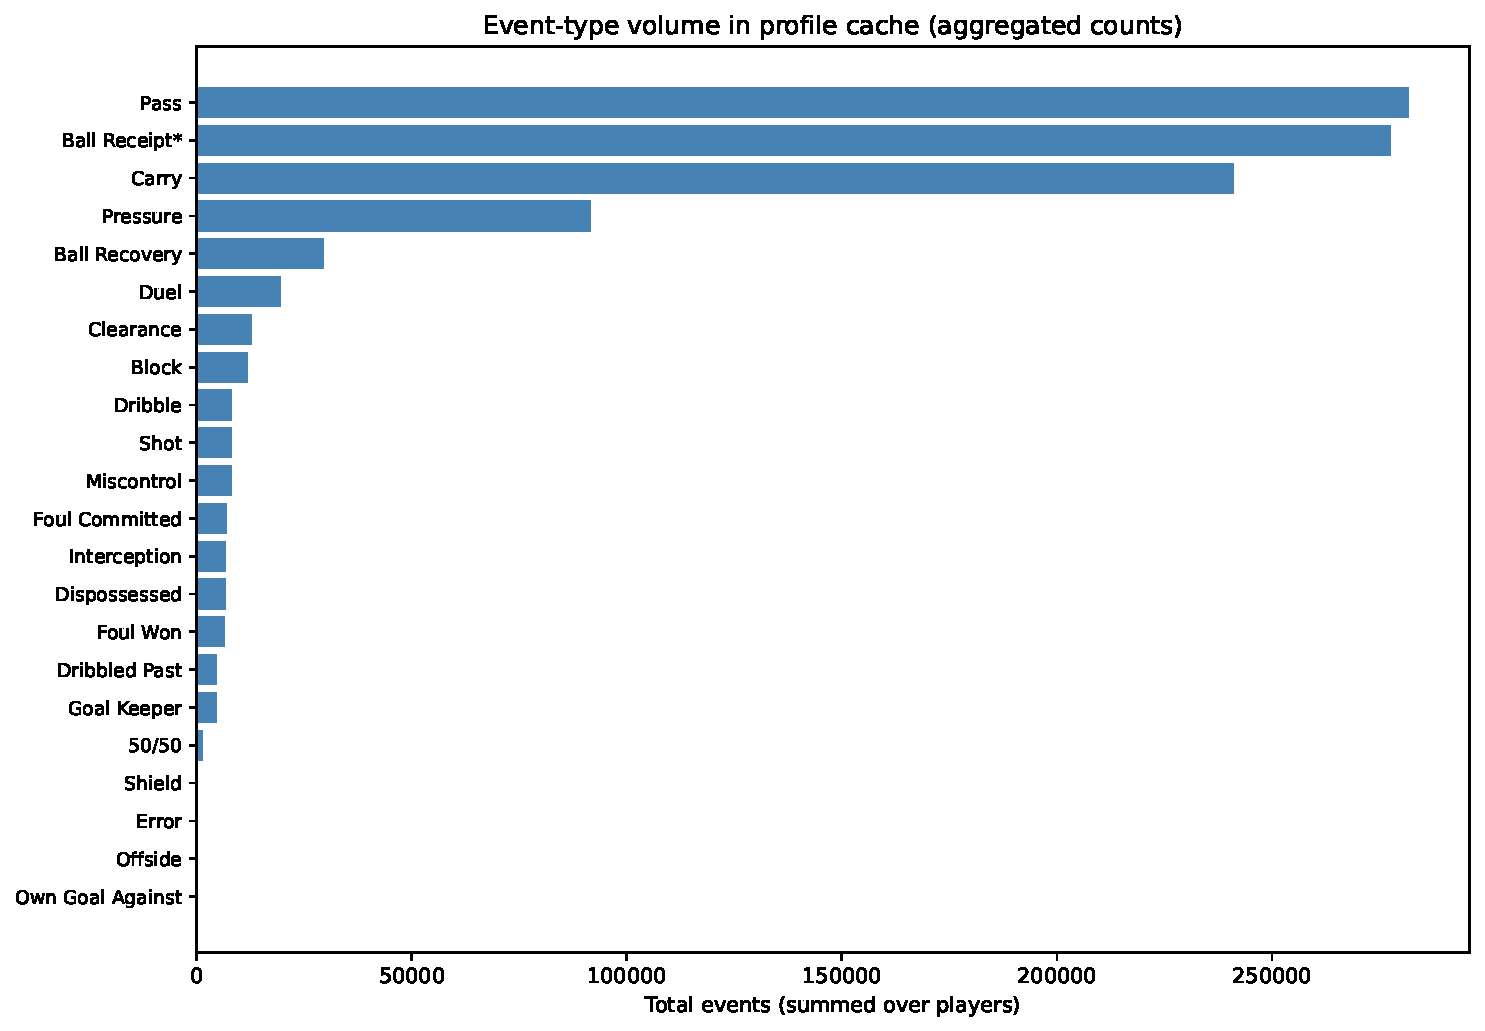
\includegraphics[width=\linewidth]{event_type_totals.pdf}
    \end{column}
    \begin{column}{0.42\textwidth}
      \footnotesize
      Top types by total events in cache:
      \begin{itemize}
        \item \texttt{Pass}: $\sim$282k
        \item \texttt{Ball Receipt*}: $\sim$278k
        \item \texttt{Carry}: $\sim$241k
        \item \texttt{Pressure}: $\sim$92k
        \item \texttt{Ball Recovery}: $\sim$29k
      \end{itemize}
      Long tail: e.g.\ \texttt{Offside}, \texttt{Own Goal Against} are rare.
    \end{column}
  \end{columns}
\end{frame}

\begin{frame}{Distribution of support $n_{p,t}$}
  \begin{columns}[T]
    \begin{column}{0.52\textwidth}
      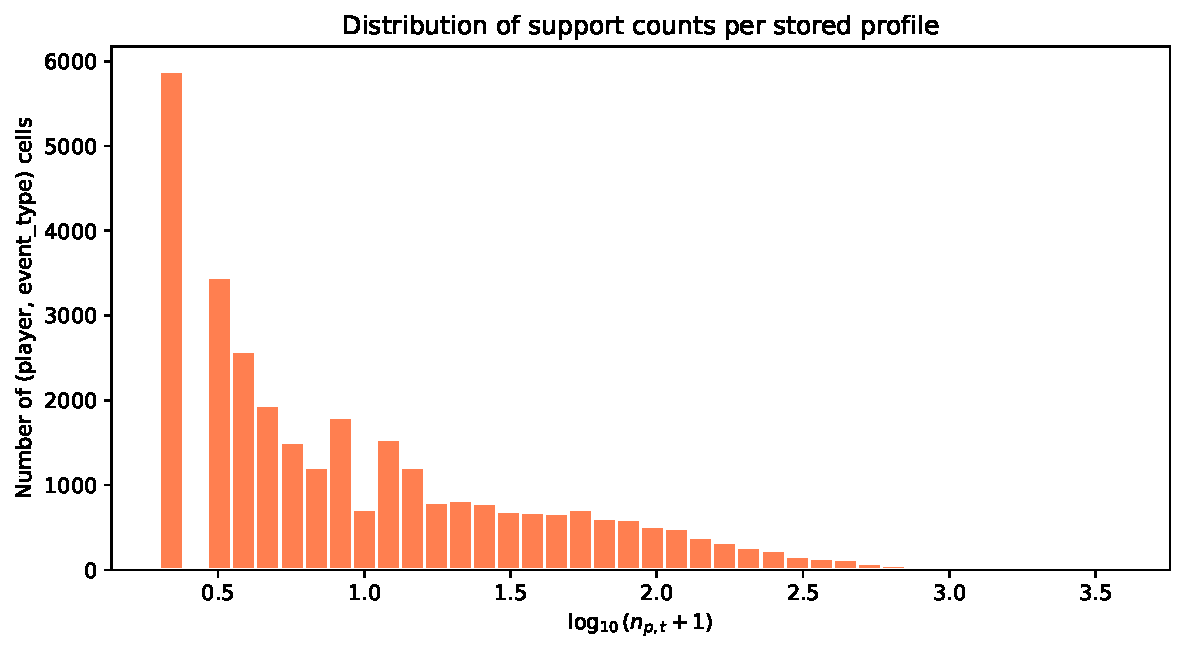
\includegraphics[width=\linewidth]{profile_count_distribution.pdf}
    \end{column}
    \begin{column}{0.46\textwidth}
      \footnotesize
      Histogram of $\log_{10}(n_{p,t}+1)$ over all stored $(p,t)$ cells.
      \vspace{0.5em}
      \begin{itemize}
        \item Many cells have moderate counts; tail reflects frequent types (e.g.\ \texttt{Pass}) for active players.
        \item Use \texttt{--min-count} at query time to ignore unstable estimates.
      \end{itemize}
    \end{column}
  \end{columns}
\end{frame}

\begin{frame}[fragile]{Worked example: query output (abridged)}
  \footnotesize
  Example command: \texttt{query} for a forward, \texttt{Pass}, \texttt{top-k=5}, \texttt{min-count=20}.
  \vspace{0.5em}
  % ASCII-only: lstlisting is fragile with some UTF-8 names in certain TeX setups
\begin{lstlisting}[language={},basicstyle=\ttfamily\tiny]
Top 5 similar players ... for event_type=Pass (query_count=49):
  Alexandra Morgan Carrasco (player_id=5085, sim=0.9850, count=75)
  Borja Iglesias Quintas (player_id=11391, sim=0.9844, count=74)
  Harry Kane (player_id=10955, sim=0.9913, count=21)
  Aitana Bonmati Conca (player_id=15284, sim=0.9899, count=37)
  Alphonso Davies (player_id=12365, sim=0.9899, count=22)
\end{lstlisting}
  \vspace{0.3em}
  \footnotesize
  \texttt{sim}: cosine similarity in $[0,1]$; \texttt{count}: $n_{p,\text{Pass}}$ for that neighbor.
\end{frame}

\begin{frame}{Worked example: interpreting neighbors}
  \begin{itemize}
    \item Under \textbf{Pass}, neighbors can span leagues and genders --- the model encodes \emph{event + 360 context}, not demographics.
    \item High \texttt{sim} with diverse names is expected if the embedding space clusters ``how'' the pass looks, not ``who''.
    \item Always check \texttt{count}: prefer $\texttt{min-count} \geq 20$--$50$ for stable rankings.
  \end{itemize}
\end{frame}

\begin{frame}{Comparison: \texttt{query} vs.\ \texttt{query-global}}
  \begin{table}
    \centering
    \footnotesize
    \begin{tabular}{p{0.28\textwidth}p{0.62\textwidth}}
      \toprule
      Mode & What it compares \\
      \midrule
      \texttt{query} & $\mathbf{v}_{q,t}$ vs.\ $\mathbf{v}_{p,t}$ for fixed $t$ (event-type conditioned). \\
      \texttt{query-global} & Whole-player vector from \texttt{player\_embeddings.pt} (mixed behaviors). \\
      \bottomrule
    \end{tabular}
  \end{table}
  Use event-type queries for ``who passes like X?''; use global for overall style similarity.
\end{frame}

\begin{frame}{Limitations / next steps}
  \begin{itemize}
    \item \textbf{Mean pooling} over all $t$-events may mix sub-styles (e.g.\ build-up vs.\ final-third passes).
    \item \textbf{Checkpoint alignment:} \texttt{feature\_vocab} and weights must come from the same \texttt{event\_encoder\_mam.pt}.
    \item \textbf{Extensions:} trimmed mean, per-league normalization, or sub-type facets (e.g.\ \texttt{pass.height.name}) --- not in current CLI.
  \end{itemize}
\end{frame}

\begin{frame}{Summary}
  \begin{itemize}
    \item \textbf{Method:} EventEncoder $\rightarrow$ per-$(p,t)$ mean $\mathbf{v}_{p,t}$ $\rightarrow$ cosine top-$k$ with count thresholds.
    \item \textbf{Implementation:} Modular PyTorch + streaming JSONL; cache $\sim$31k $(p,t)$ cells from $\sim$1.03M events.
    \item \textbf{Figures:} Event-type totals and distribution of $n_{p,t}$ (\texttt{figures/}, regenerate via \texttt{scripts/generate\_slide\_figures.py}).
  \end{itemize}
\end{frame}

\end{document}
